

%\documentclass[12pt]{report}

\documentclass[12pt]{article}
%\usepackage{natbib}  % used for citations
\usepackage[parfill]{parskip} %used for formatting style of text



\usepackage{graphicx,fancyhdr}
\usepackage{amssymb,amsmath}
\usepackage{epigraph,fancyvrb,eqparbox}
\usepackage[multiple]{footmisc}
\usepackage{menukeys}
\usepackage{menukeys}
\usepackage{url}
\usepackage[colorlinks = true, linkcolor = blue, urlcolor = blue]{hyperref}
\usepackage{setspace}

\pagestyle{fancyplain}

%\usepackage{hyperref}
%\usepackage{epsf,psfig,graphicx,fancyheadings}
% \textwidth 7in
% \textheight 9in
% \oddsidemargin 0in
% \topmargin -.25in

%-----------------------------------------------
% The following settings are from Dr. Davidian's
% ST810A Handout on Advanced LaTeX Features

%\setlength{\paperheight}{11.0in}
%\setlength{\paperwidth}{8.5in}

%%%%%%%%%%%%%%%%%%%%%%%%%%%%%%%%%%%%%%%%%%%%%%%%%
% For Desktop @ CalPoly (for Postscript)

%\setlength{\oddsidemargin}{0.5in}
%\setlength{\evensidemargin}{0.5in}
%\setlength{\topmargin}{-.5in}

%%%%%%%%%%%%%%%%%%%%%%%%%%%%%%%%%%%%%%%%%%%%%%%%%
% For Laptop @ Calpoly (for Postscript)

% \setlength{\oddsidemargin}{0.in}
% \setlength{\evensidemargin}{0.in}
% \setlength{\topmargin}{0.25in}

%%%%%%%%%%%%%%%%%%%%%%%%%%%%%%%%%%%%%%%%%%%%%%%%%
% For Desktop @ CalPoly (for PDF)

%\setlength{\oddsidemargin}{0.in}
%\setlength{\evensidemargin}{0.in}
%\setlength{\topmargin}{-.5in}
%
%%%%%%%%%%%%%%%%%%%%%%%%%%%%%%%%%%%%%%%%%%%%%%%%%%
%% For Laptop @ Calpoly (for PDF)
%
%% \setlength{\oddsidemargin}{0.in}
%% \setlength{\evensidemargin}{0.in}
%% \setlength{\topmargin}{0.25in}
%
%
%
%\setlength{\oddsidemargin}{0.0in}
%\setlength{\topmargin}{-0.5in}
%\setlength{\headheight}{0.20in}
%\setlength{\headsep}{3ex}
%\setlength{\baselineskip}{2ex}
%\setlength{\textheight}{9in}
%\setlength{\textwidth}{6.4in}
%\renewcommand{\baselinestretch}{1.1}

% Sets margins to 1 in
\addtolength{\oddsidemargin}{-.5in}%
\addtolength{\evensidemargin}{-.5in}%
\addtolength{\textwidth}{1in}%
\addtolength{\textheight}{1.3in}%
\addtolength{\topmargin}{-.8in}%

%\setlength{\headheight}{0.20in}
%\setlength{\headsep}{3ex}
%\setlength{\headrulewidth}{0.2pt}
%\setlength{\footrulewidth}{0.15pt}
%\setlength{\parskip}{2.3ex}
% %set to no indentation
%\setlength{\parindent}{0.0in}
%\setlength{\baselineskip}{2ex}
%\setlength{\textheight}{9.in}
%\setlength{\textwidth}{6.5in}

\def \doublespace{\openup 2\jot}
% For double or 1.5 spacing
%\renewcommand{\baselinestretch}{1.5}
\tolerance=500

\def\boxit#1{\vbox{\hrule\hbox{\vrule\kern6pt
\vbox{\kern6pt#1\kern6pt}\kern6pt\vrule}\hrule}}
\renewcommand{\theequation}{\thesection.\arabic{equation}}
% The following for TOC
%\renewcommand{\thepage}{\roman{page}}
% to be followed by this for the main text
\renewcommand{\thepage}{\arabic{page}}


%-----------------------------------------------

%%%%%%%%%%%%%%%%%%%%%%%%%%%%%%%%%%%%%%
%Define any shortcut aliases below

\newtheorem{theo}{Theorem}[section]

\newenvironment{note}{\begin{quote}\emph{Note:\ }}{\end{quote}}
\newenvironment{defn}{
\begin{description}
\item[Definition ]}
{\end{description}}

\newenvironment{ttscript}[1]{%
    \begin{list}{}{%
    \settowidth{\labelwidth}{\texttt{#1}}
    \setlength{\leftmargin}{\labelwidth}
    \addtolength{\leftmargin}{\labelsep}
    \setlength{\parsep}{0.5ex plus0.2ex minus0.2ex}
    \setlength{\itemsep}{0.3ex}
    \renewcommand{\makelabel}[1]{\texttt{##1\hfill}}}}
    {\end{list}}

\newcommand{\bt}{\begin{tabular}}
\newcommand{\et}{\end{tabular}}
\newcommand{\bc}{\begin{center}}
\newcommand{\ec}{\end{center}}
\newcommand{\bi}{\begin{itemize}}
\newcommand{\ei}{\end{itemize}}
\newcommand{\be}{\begin{enumerate}}
\newcommand{\ee}{\end{enumerate}}
\newcommand{\bq}{\begin{quote}}
\newcommand{\eq}{\end{quote}}
\newcommand{\vect}[1]{\mbox{\boldmath $ #1$}}
\newcommand{\avg}[1]{$\overline{#1}$}
\newcommand{\bmp}{\begin{minipage}}
\newcommand{\emp}{\end{minipage}}
\newcommand{\hr}{\u{\hspace{7in}}}
\newcommand{\sr}{\u{\hspace{5in}}}
\newcommand{\chs}{\chi^2}

\newcommand{\labn}[1]{\Large{\textbf{\fbox{Lab #1}}}\hspace{0.1in} \normalsize{\emph{Some of these problems may be more challenging than others. Please feel free to work with others, attend office hours, or post on the course discussion forum if you need help.  While collaboration with other students is encouraged, each student is responsible for submitting his or her own work.  This assignment should be submitted in one well-commented SAS program.  For any questions that require a written answer, do so in the SAS comments.  Be sure to re-name the uploaded SAS scripts according to the naming convention}} \texttt{LastnameFirstinitial\textunderscore Lab\#.sas} (\emph{e.g.,} \texttt{PileggiS\textunderscore Lab#1.sas}).}


\newcommand{\hd}[1]{\lhead{STAT 330/530: Lab #1}\rhead{Pileggi, FA17}}
\newcommand{\bs}{\underline{\hspace{0.5in}}}

%\newcommand{\bv}{\footnotesize
%\bmp{.5\textwidth}
%\begin{Verbatim}[frame=single,label=SAS Code,commandchars=\\\{\}],xrightmargin=.5\textwidth}
%
%\newcommand{\ev}{\end{Verbatim}
%\emp
%\normalsize}

\newcommand{\bv}{\begin{code}}
\newcommand{\ev}{\end{code}}

 \newenvironment{code}[1]%
  {\vspace{.1in}\footnotesize\Verbatim[frame=single,label=SAS Code,commandchars=\\\{\},xrightmargin=#1\textwidth,framesep=.2in,labelposition=all]}
  {\endVerbatim\normalsize}

\newenvironment{craw}[2]%
{\vspace{.1in}\footnotesize\Verbatim[frame=single,label=#2,commandchars=\\\{\},xrightmargin=#1\textwidth,framesep=.2in,labelposition=all]}
  {\endVerbatim\normalsize}

\newenvironment{cbox}[1]%
{\vspace{.1in}\footnotesize\Verbatim[frame=single,commandchars=\\\{\},xrightmargin=#1\textwidth,framesep=.2in,labelposition=all]}
  {\endVerbatim\normalsize}

\newcommand{\head}[1]{\large \textbf{#1} \normalsize}

\newcommand{\ttt}[1]{\textbf{\texttt{#1}}}


\newcommand{\bsval}[1]{\underline{\hspace{0.2in}{[#1]}\hspace{0.2in}}}

\newcommand{\ttb}{\textbf}
\newcommand{\tte}{\emph}
\newcommand{\ttu}{\underline}



\newcommand{\jdhr}{\vspace{0.2in}\hrule}


\newcommand{\uspace}[1]{\underline{\hspace{#1}}}

\newenvironment{ident}{\begin{list}{}{}
         \item[]}{\end{list}}

\newenvironment{proposition}{
\begin{description}
\item[Proposition: ]}
{\end{description}}

\newcommand{\bpr}{\begin{proposition}}
\newcommand{\epr}{\end{proposition}}



% \newenvironment{example}
%     {
%         \begin{list}{\textbf{Example:}}
%         {
%         \settowidth{\labelwidth}{}
%         \setlength{\leftmargin}{\labelwidth}
%         }
%     }
%     {\end{list}}


\newenvironment{example}{
\jdhr \vspace{-.17in}\jdhr
\textbf{Example: }}
{}

\newcommand{\bex}{\begin{example}}
\newcommand{\eex}{\end{example}}

\newenvironment{onyourown}{
\jdhr \vspace{-.17in}\jdhr
\textbf{On Your Own: }}
{}

\newcommand{\boy}{\begin{onyourown}}
\newcommand{\eoy}{\end{onyourown}}


%\newenvironment{debug}{
%\jdhr \vspace{-.17in}\jdhr
%\ttb{Debug the Code}
%\fbox{
%\bmp{.95in}
%\includegraphics[height=.35in]{C:/images/bug4.jpg}\includegraphics[height=.35in]{C:/images/buggy8.jpg}
%\emp}
%}
%{\jdhr}

\newenvironment{debug}{
\jdhr \vspace{-.17in}\jdhr
\ttb{Debug the Code: }
\fbox{
\bmp{.95in}
\includegraphics[height=.35in]{C:/images/bug4.jpg}\includegraphics[height=.35in]{C:/images/mushi90.jpg}
\emp}
}
{}


\newcommand{\bbug}{\begin{debug}}
\newcommand{\ebug}{\end{debug}}


\begingroup
  \catcode `_=11
  \gdef\myuscore{_}
  \catcode `~=11
  \gdef\mytilde{~}
  \catcode `\|=0
  \catcode `\\=11
  |gdef|mybs{\}
|endgroup

%Define any shortcut aliases above


%....................................................................
%....................................................................
%....................................................................
%....................................................................
%....................................................................
%....................................................................
%....................................................................
%....................................................................



\usepackage{amssymb}
				

\begin{document}
\hd{15}
\labn{15}
\vskip10pt

\noindent Recall Lab 14 where you created a table of descriptive statistics of the 2012 Olympic Medalists by country using the \ttt{O2012.sas7bdat} data set (this data set name starts with an ``oh'' and not a zero).  In this lab, you are going to follow a series of steps to re-create that table using \ttt{PROC TABULATE}.  Skip to page 4 to see an example table.
 \begin{enumerate}
\item In a comment in your SAS code, briefly describe the programming approach you took to create the table displayed on page 3 in Lab 14.
\begin{enumerate}
\item What actions did you do in data steps?
\item What actions did you do in procedures?
\end{enumerate}
\item In a comment in your SAS code, briefly describe your game plan for creating this table with \ttt{PROC TABULATE}.
\begin{enumerate}
\item What actions will you need to do in data steps?
\item What actions will you need to do you do in procedures?
\item Briefly, describe the \emph{structure} of the table that you want to create.
\begin{enumerate}
\item What is the table dimension?
\item What goes on the rows, columns, and pages?
\end{enumerate}
\end{enumerate}
\item Create a SAS library to access the \ttt{O2012.sas7bdat}.
\item Follow the subsequent steps to establish the \emph{structure} of the table from Lab 14 using \ttt{PROC TABULATE}.  Your goal for this question is to create the table structure by following the subsequent steps:
%\item[] 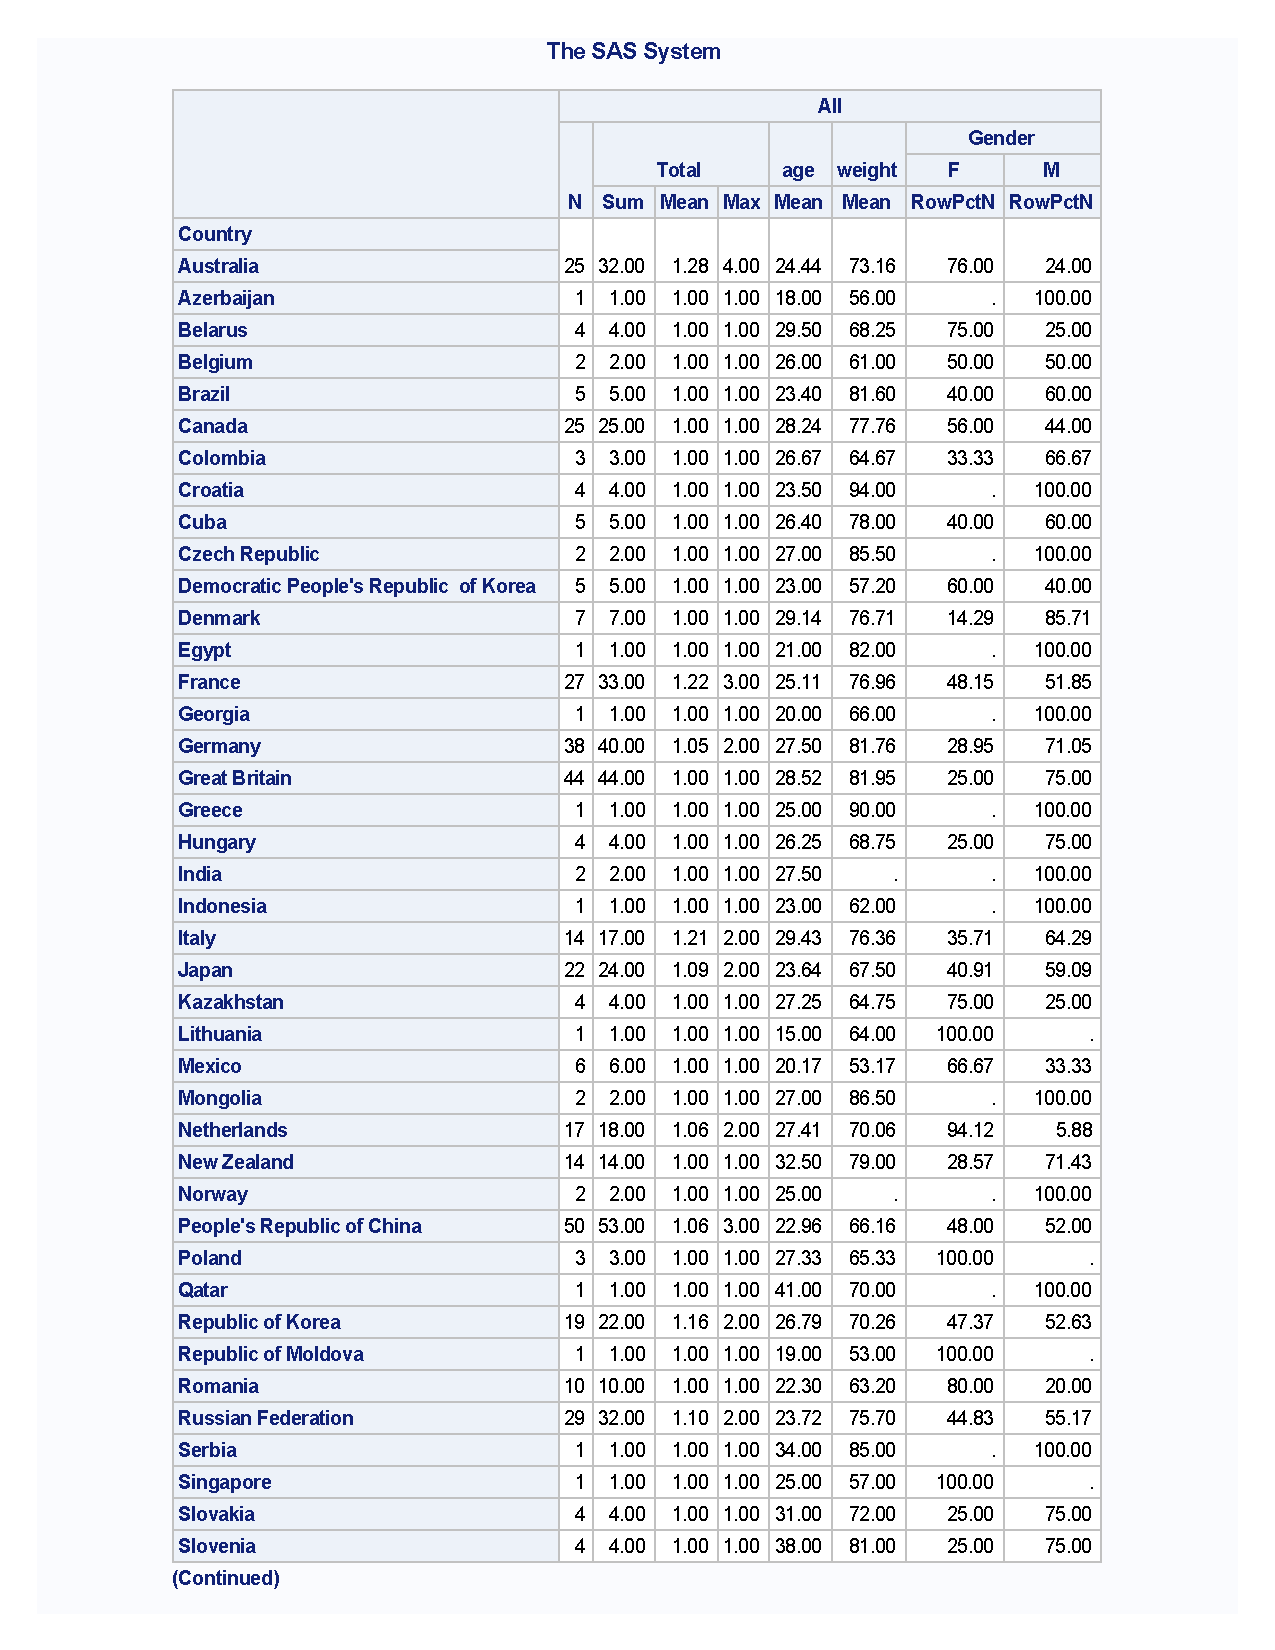
\includegraphics[trim={2cm 22.0cm 1cm 1.7cm},clip,width=1.0\textwidth]{q4e.pdf}
%\item[]
\begin{enumerate}
\item Use \ttt{PROC TABULATE} to create a table that has rows for different countries and a single column that represents the number of Olympic medalists from that country.
\item[] 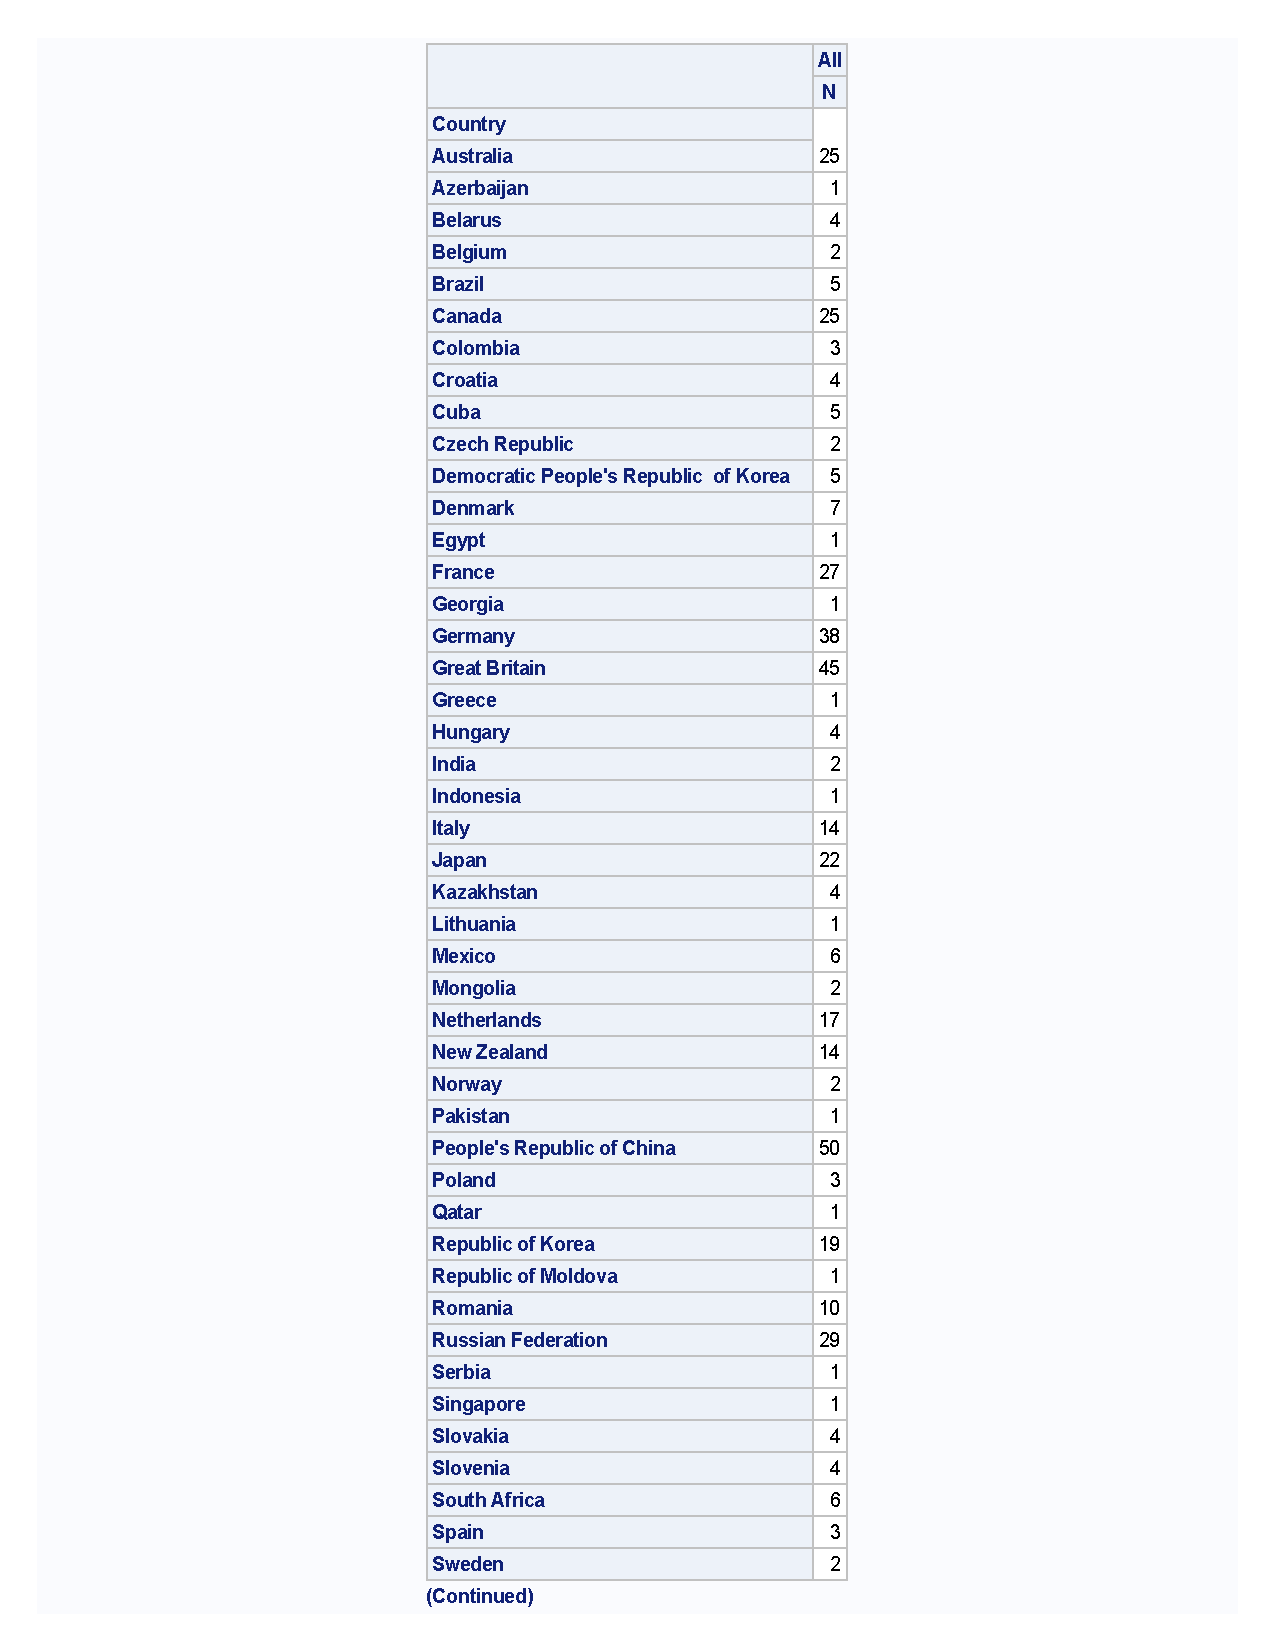
\includegraphics[trim={3cm 24.0cm 3cm 0cm},clip,width=1.0\textwidth]{q4a.pdf}
\item Copy and paste your SAS code from the previous step.  Modify this code so that the table now has an additional column that represents the sum of the total number of medals won by that country.
\item[] 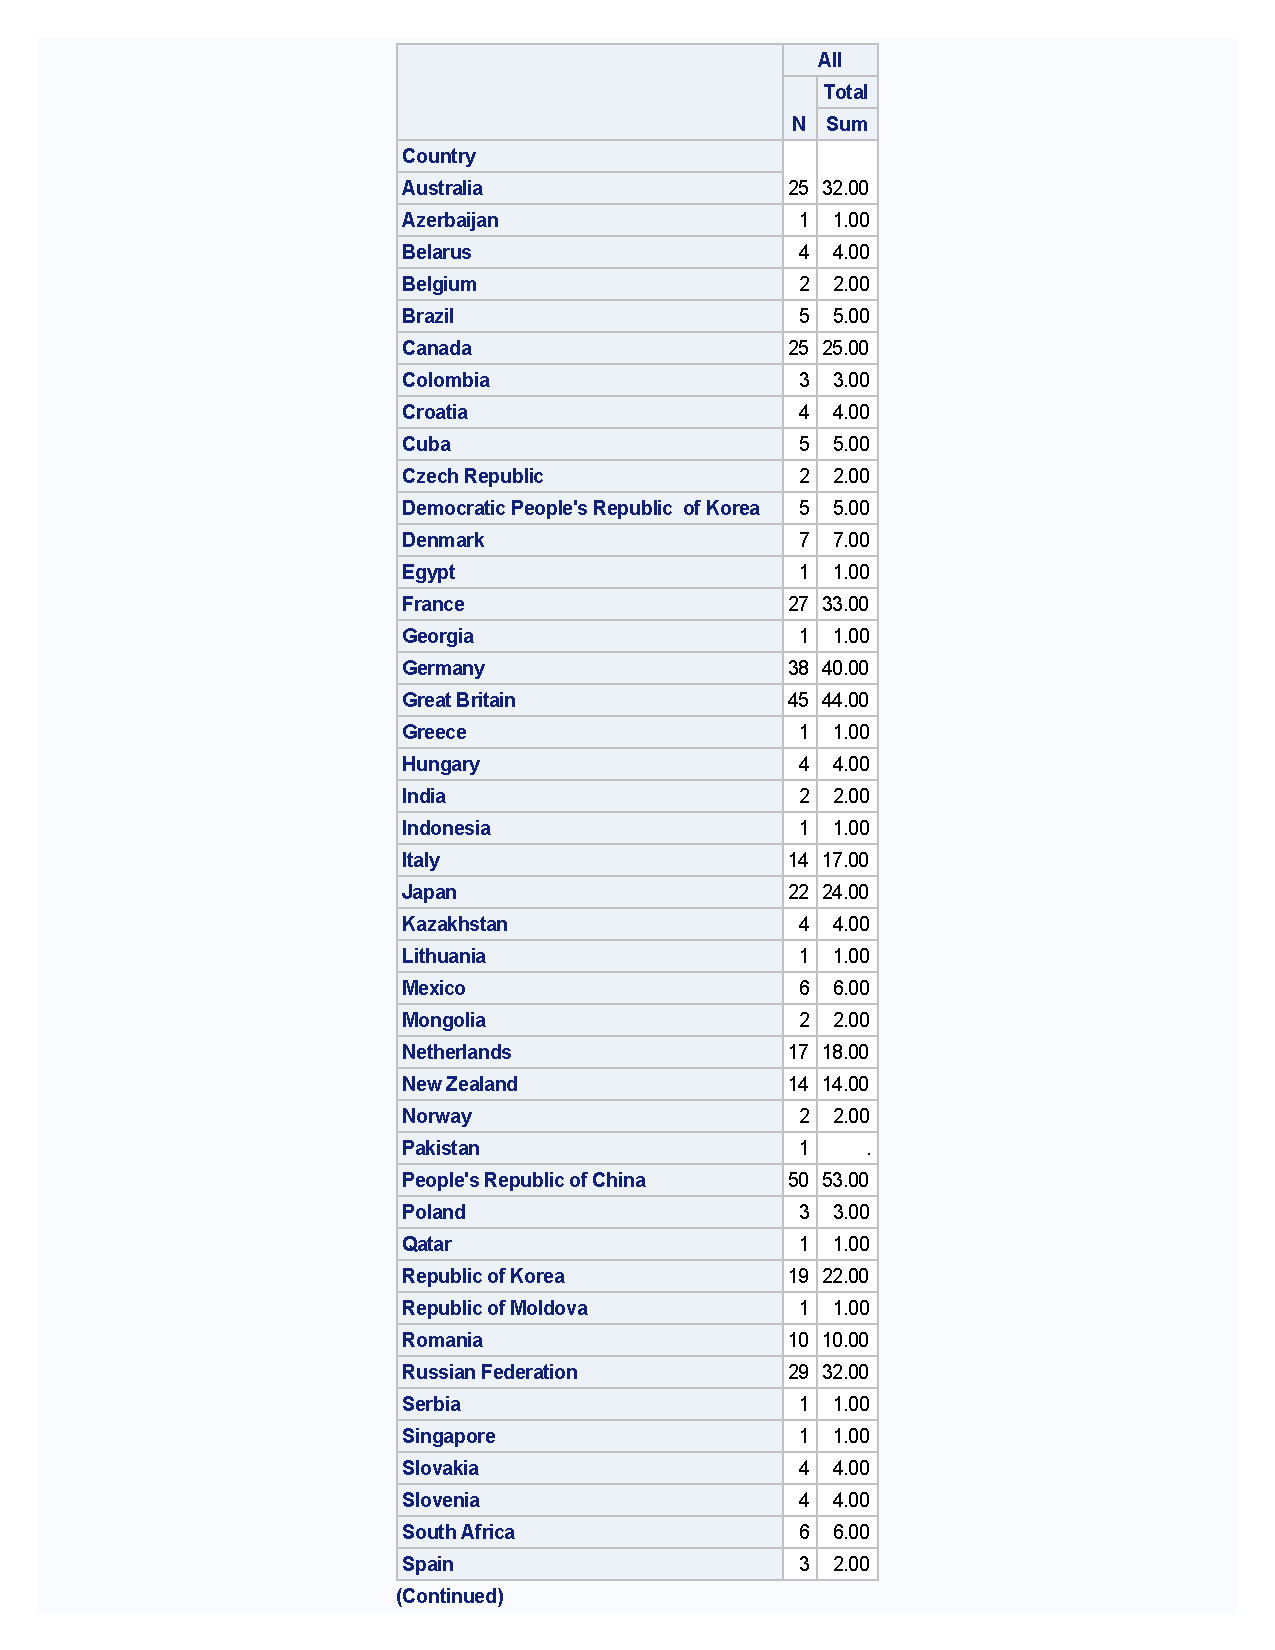
\includegraphics[trim={3cm 24.0cm 3cm 0cm},clip,width=1.0\textwidth]{q4b.pdf}
\item Copy and paste your SAS code from the previous step.  Modify this code so that the table now has three statistics for the total number of medals: sum, average total medals won, and maximum total medals won by an athlete.  Your table now has 4 columns.
\item[] 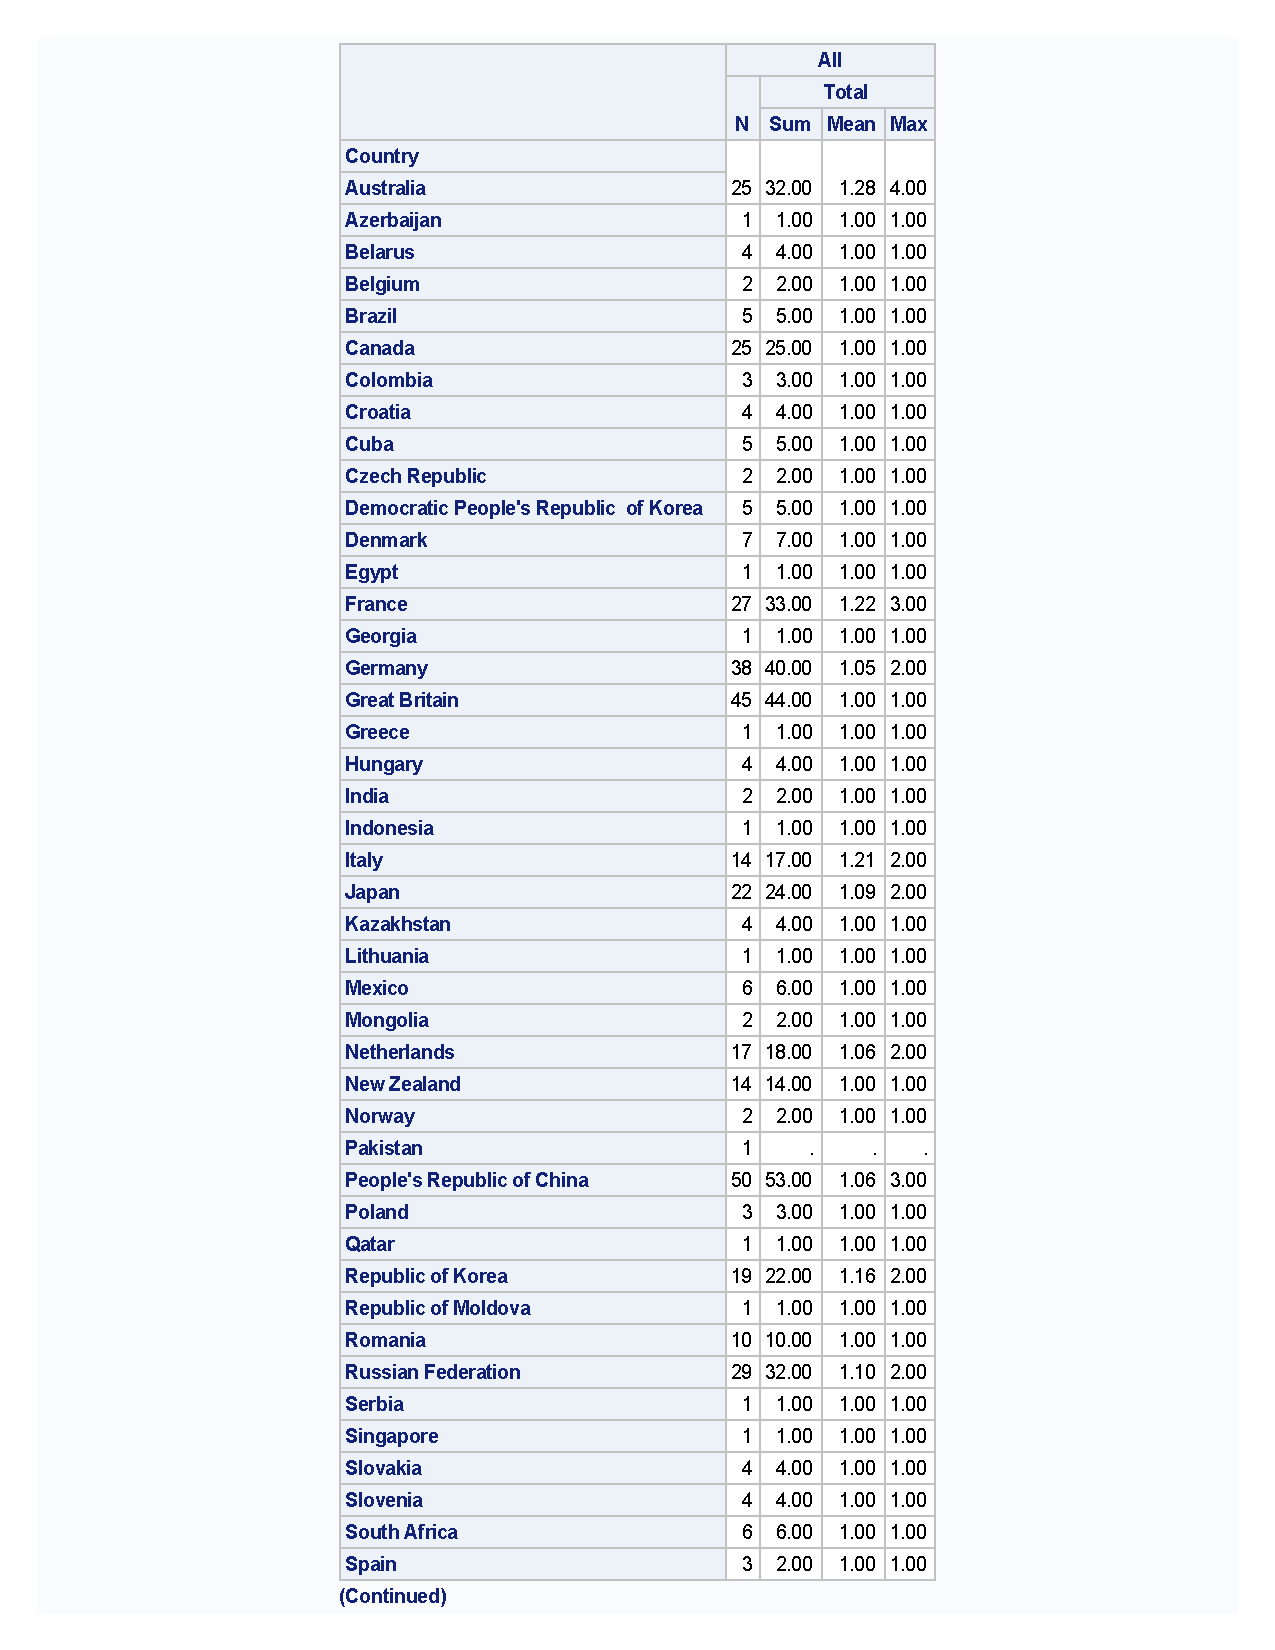
\includegraphics[trim={3cm 24.0cm 3cm 0cm},clip,width=1.0\textwidth]{q4c.pdf}
\item Copy and paste your SAS code from the previous step.  Modify this code so that the table now has two additional columns for the average age and average weight of the Olympic athletes.
\item[] 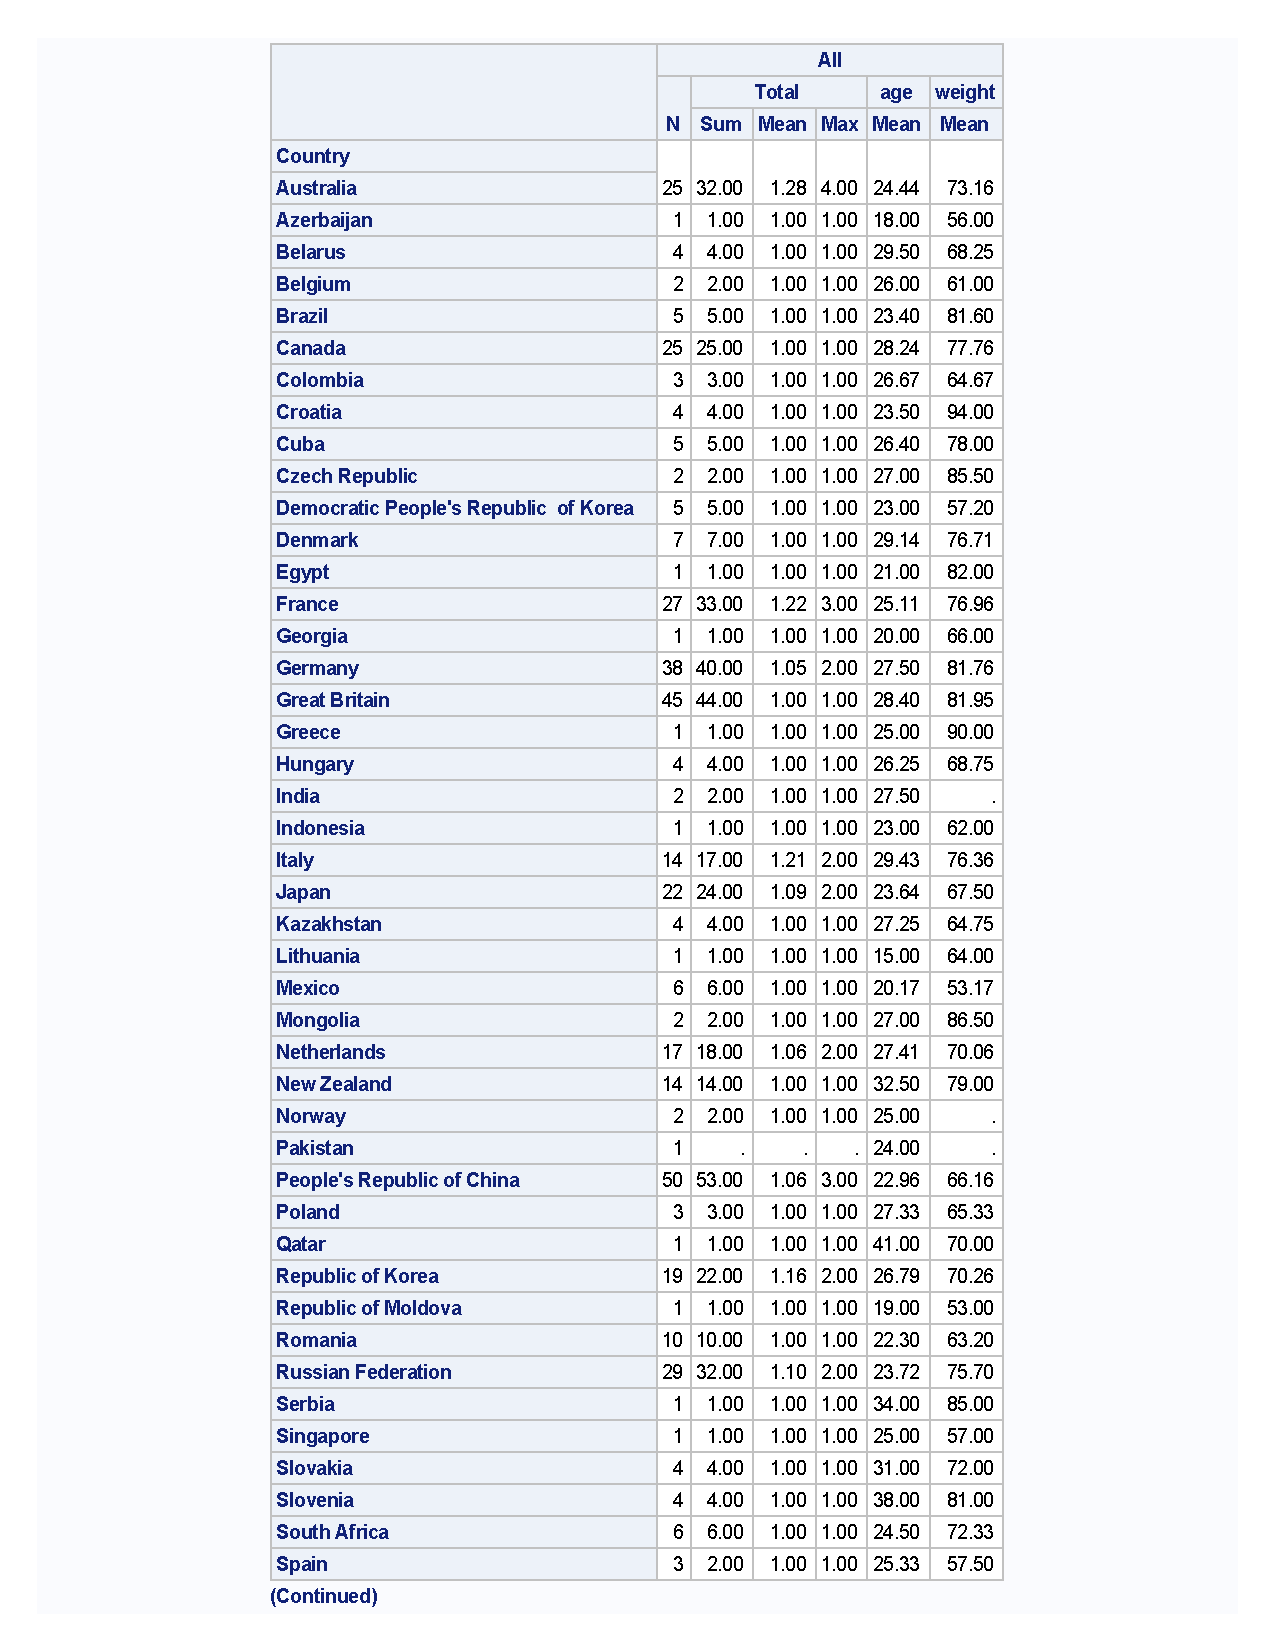
\includegraphics[trim={3cm 24.0cm 3cm 0cm},clip,width=1.0\textwidth]{q4d.pdf}    
\item Copy and paste your SAS code from the previous step.  Modify this code so that the table now has two additional columns for the percent of each country's Olympic medalists that are male and female.
\item[] 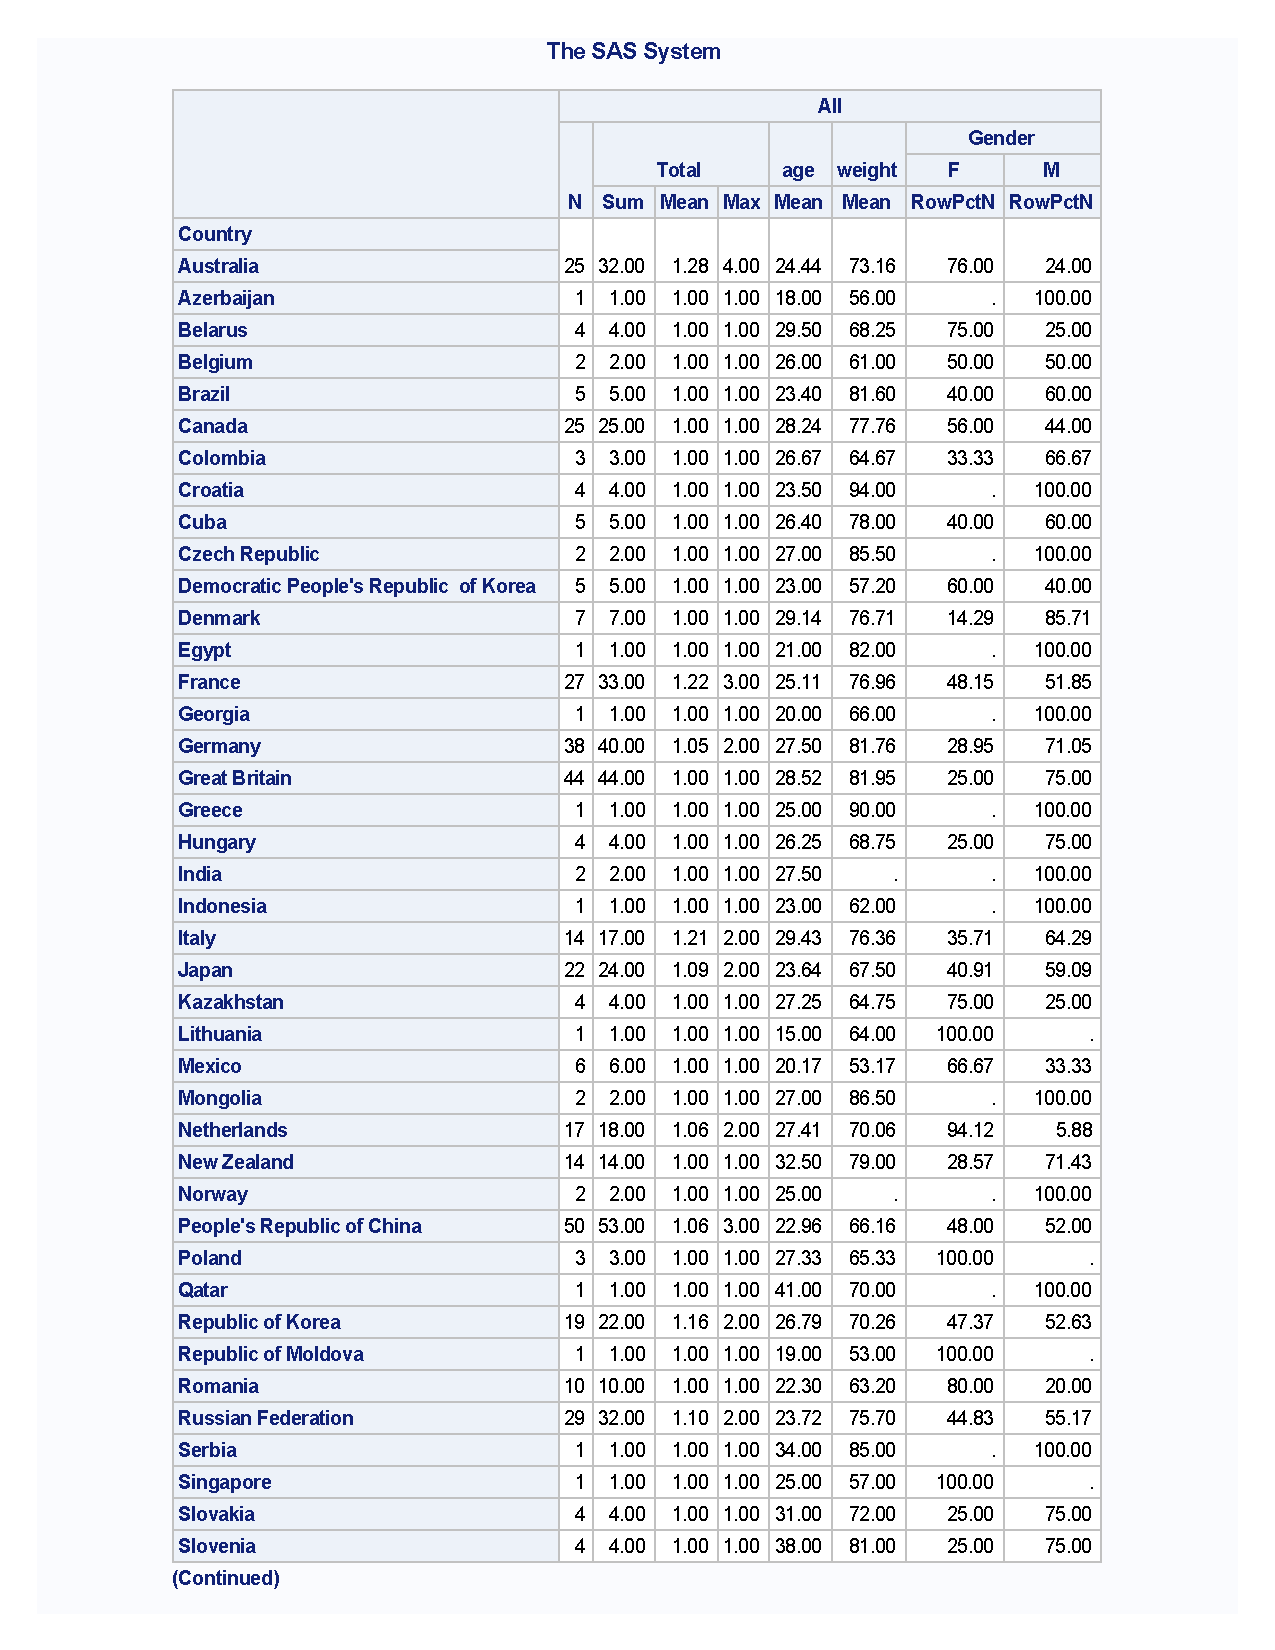
\includegraphics[trim={1cm 22.0cm 1cm 0.5cm},clip,width=1.0\textwidth]{q4e.pdf}
\end{enumerate}
\item Copy and paste your SAS code from the previous step.  Modify this code so that the table \emph{header} appears as below (you will \emph{format variable values} in the next step).  This requires using various forms of labels.
\item[] 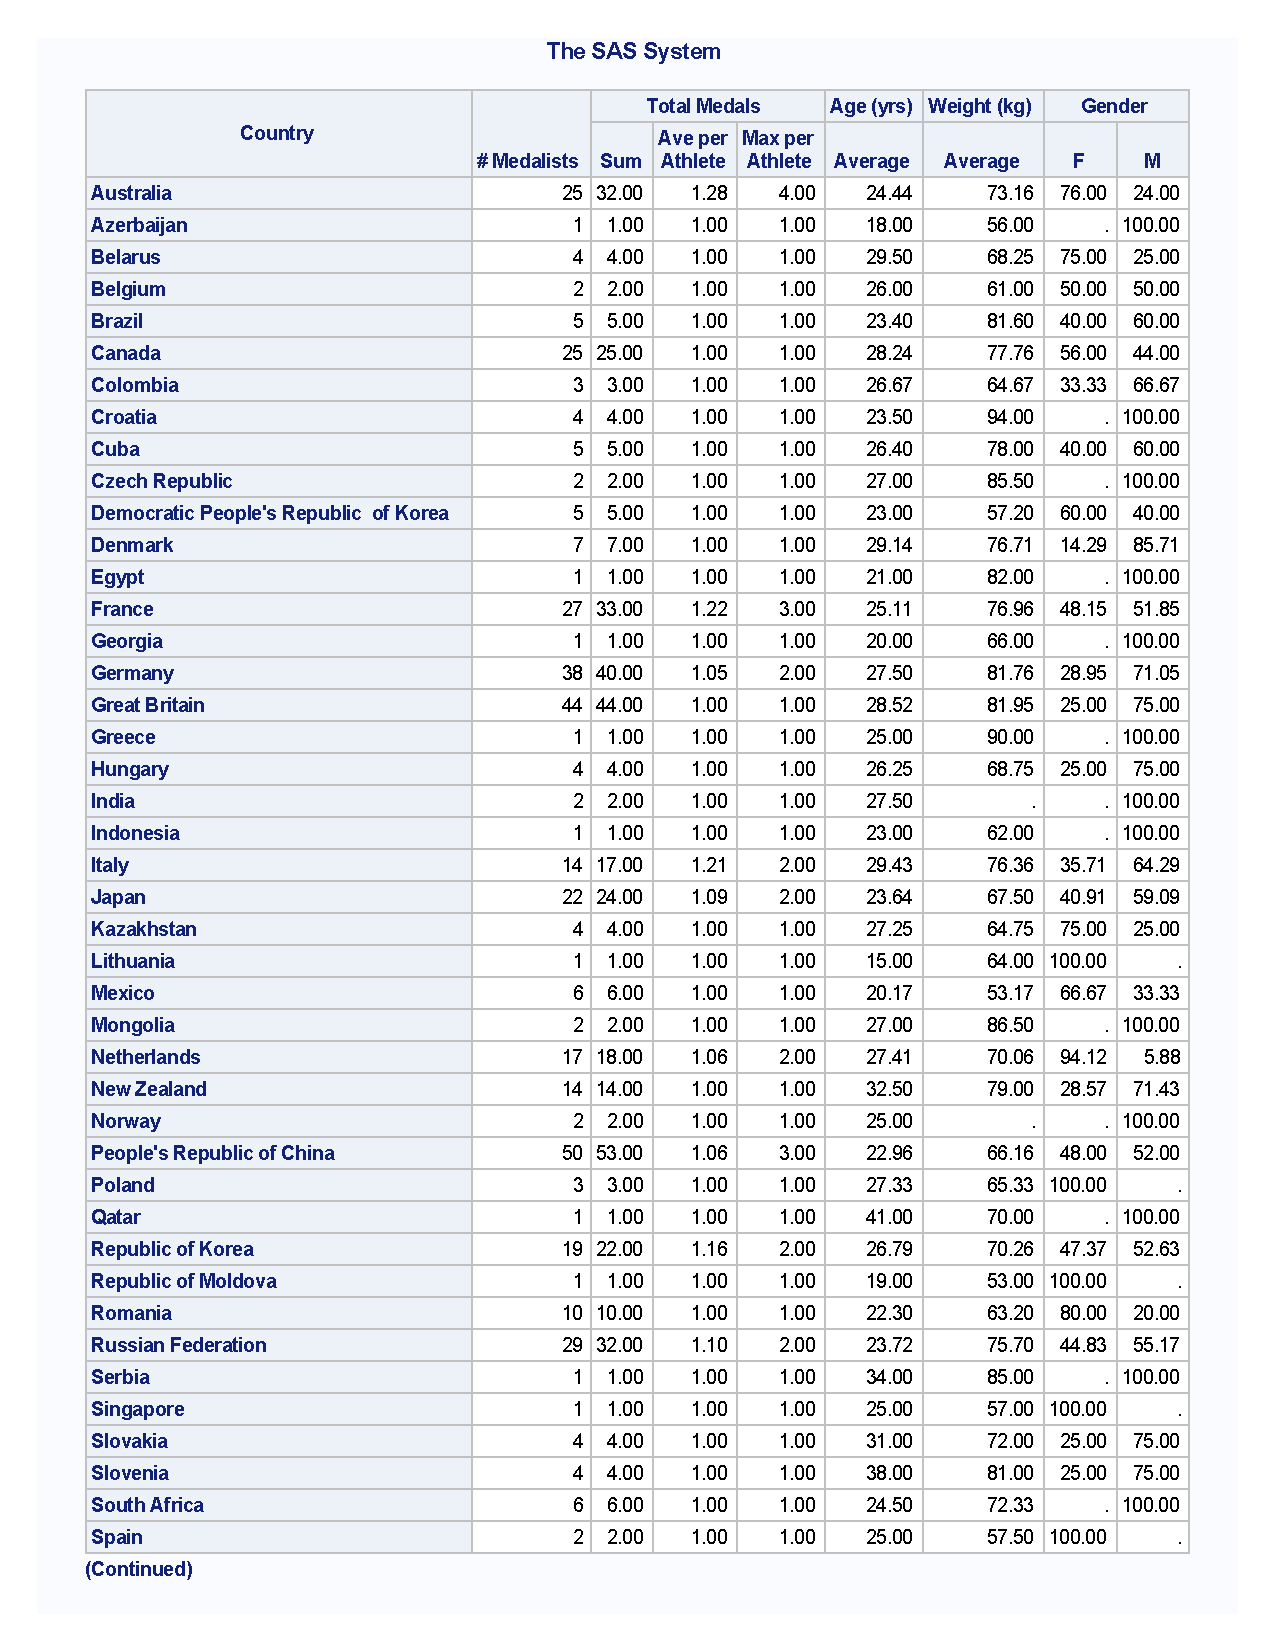
\includegraphics[trim={1cm 22.0cm 1cm 0.5cm},clip,width=1.0\textwidth]{q5.pdf}
\item Copy and paste your SAS code from the previous step.  Follow the subsequent steps to modify this code to \emph{format variable values} so that they appear as below.
\begin{enumerate}
    \item Apply the following formats to variable values:
    \item[]
    \begin{tabular}{rl}
    %statistic & display \\
    sum of total medals & no decimal places \\
    average of total medals & two decimal places \\
    max of total medals & no decimal places \\
    average age & one decimal place \\
    average weight & one decimal place \\
    \end{tabular}
    \item Create and apply a format for gender such values display as ``Female'' and ``Male''. %\emph{Hint: When creating and apply formats for a character variable, you need to use a dollar sign (\$).}
    \item Create and apply a picture format for percent such that percents display as rounded to one decimal place with a percent sign.  %\emph{Hint: Review Example 8 in the supplemental SAS code provided with Lecture 16.}
    \item Change the display of missing values from period (.) to three horizontal dashes (``---'') by using the \ttt{MISSTEXT} \emph{option} on the \ttt{TABLE} statement.
\end{enumerate}
\item[] 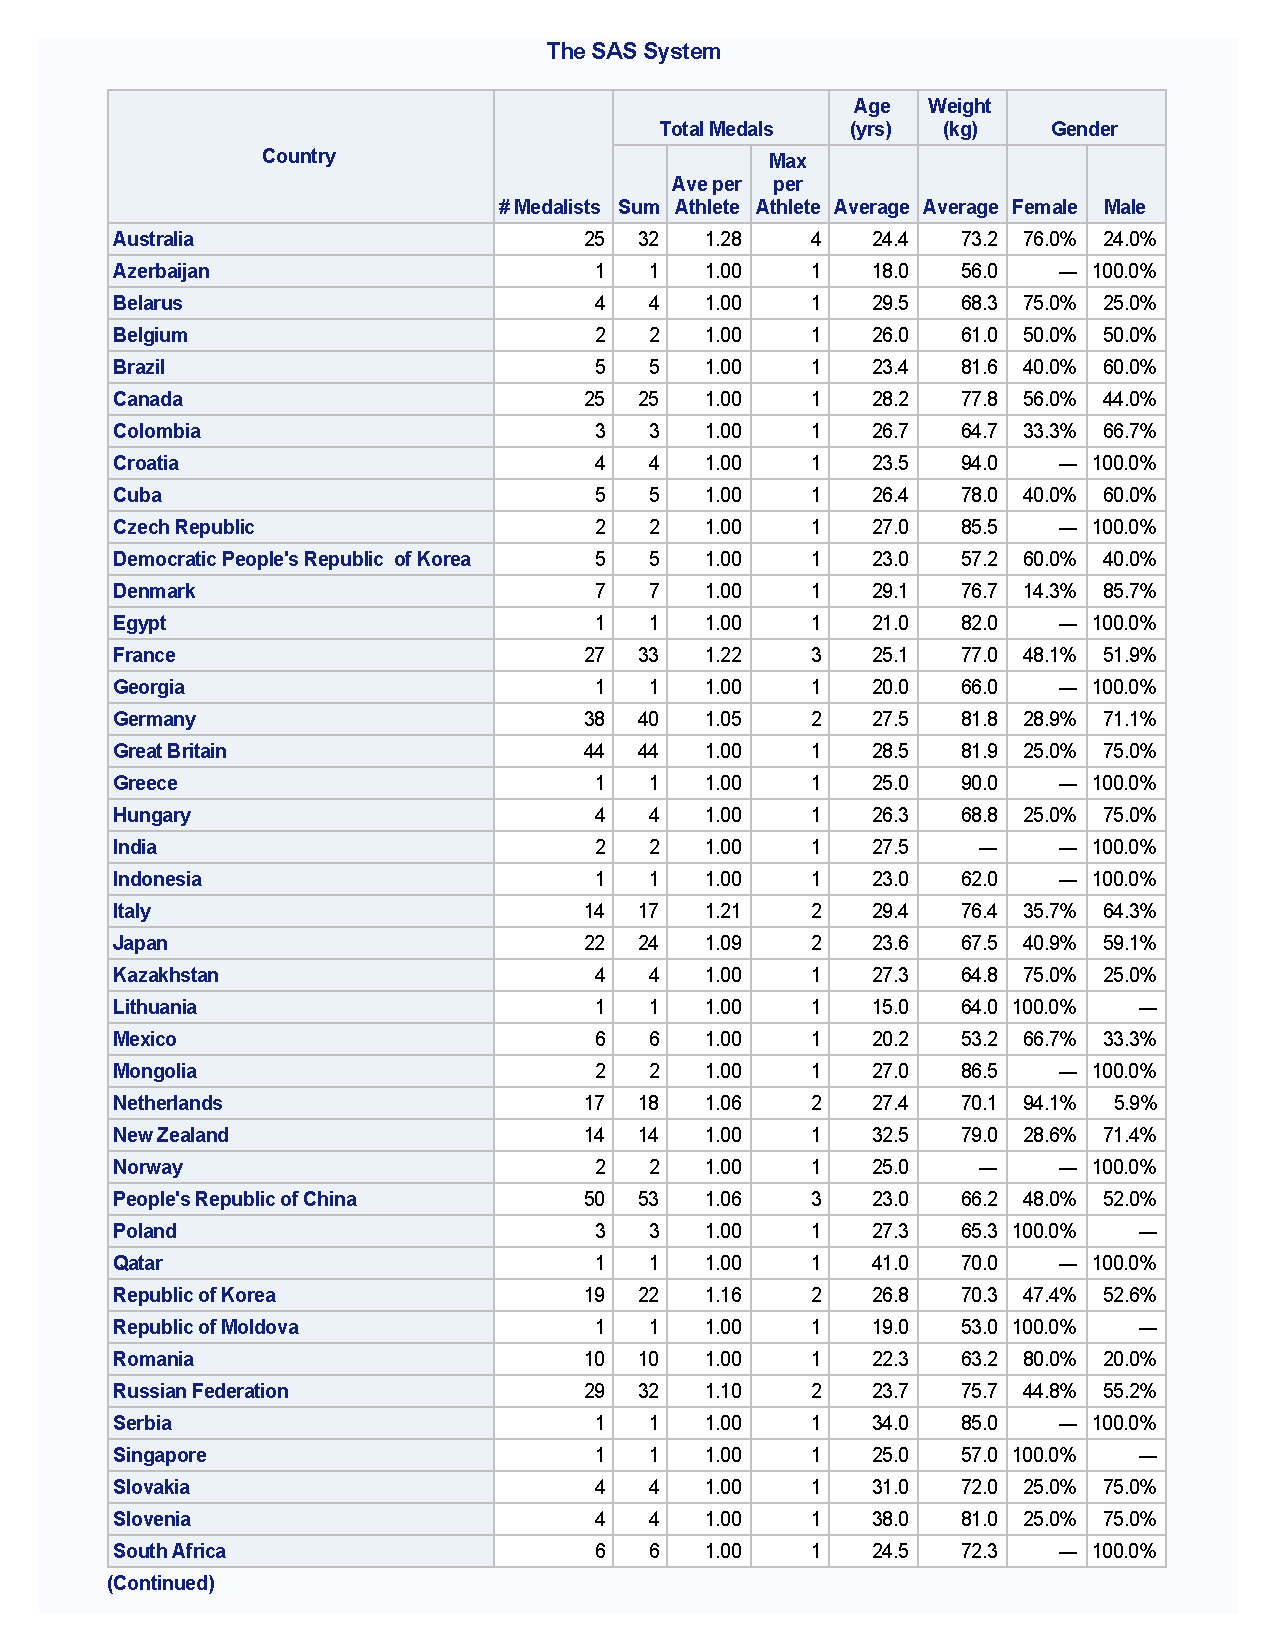
\includegraphics[trim={1cm 22.0cm 1cm 0.5cm},clip,width=1.0\textwidth]{q6.pdf}

\item Copy and paste your SAS code from the previous step.  Modify this code to highlight the background color of cells that correspond to countries with more than 20 athletes in the color of your choice.  (See last page for an example.)
\item Copy and paste your SAS code from the previous step.  Modify this code to export your table to a pdf.
\item Copy and paste your SAS code from the previous step.  Modify this code to create a macro that allows you to quickly view combinations of styles and colors as follows:
\begin{enumerate}
\item Include macro debugging options in your SAS code.
\item The macro should take two parameters: one for the \emph{style} of the pdf, and one for the \emph{color} of the highlighted cells.
\item The file name  of the pdf should indicate the \emph{style} and \emph{color} used.
\item The document title should indicate the \emph{style} and \emph{color} used.
\item Execute the macro at least three times:
\begin{enumerate}
\item \emph{Pearl} style (this is the default style), highlight color of your choice
\item new style of your choice, new highlight color of your choice
\item new style of your choice, new highlight color of your choice
\end{enumerate}
\item Open the pdfs you created.  In a comment in your SAS code, note your preferred style/color combination.  Upload these pdfs in addition to your SAS code.
\end{enumerate}
\end{enumerate}
\newpage
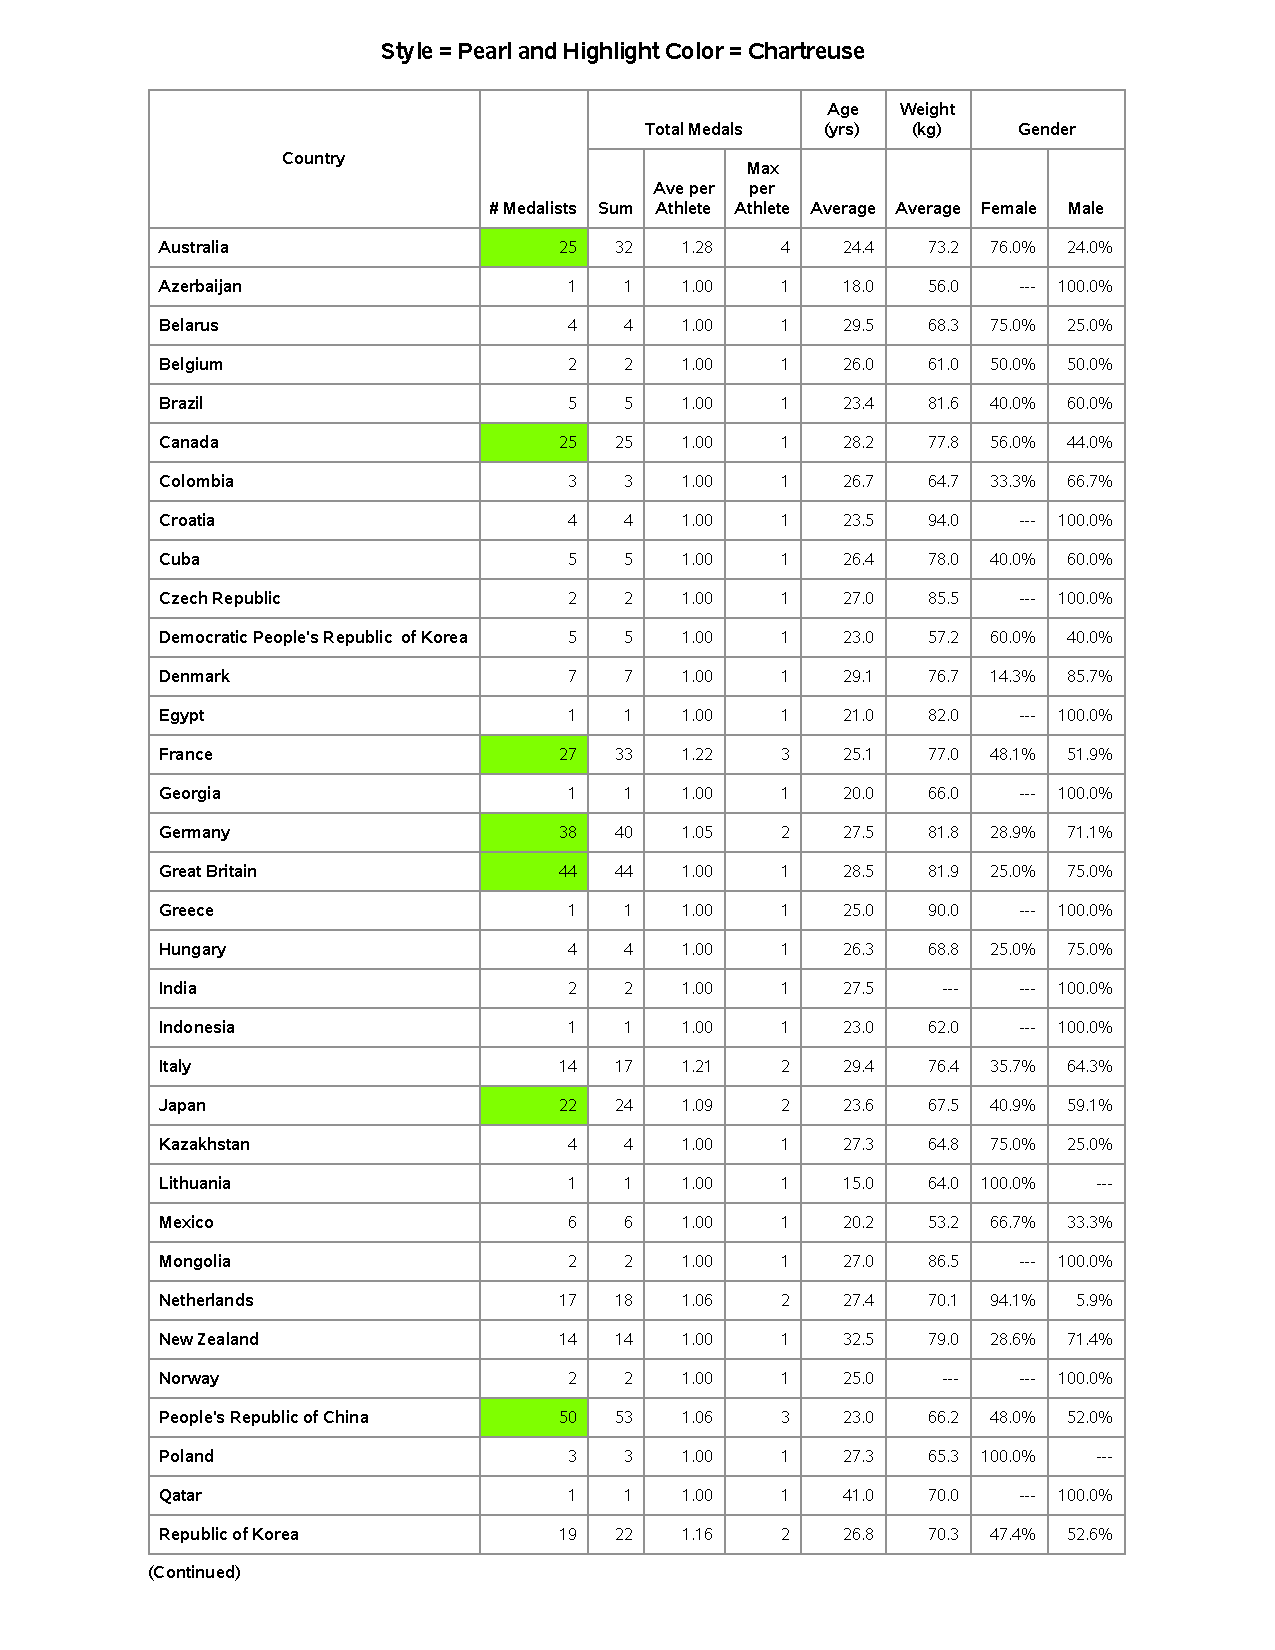
\includegraphics[trim={2cm 0cm 2cm 0cm},clip,width=0.95\textwidth]{Lab15table_Chartreuse_Pearl.pdf}
\end{document} 